%% For double-blind review submission, w/o CCS and ACM Reference (max submission space)
\documentclass[sigplan]{acmart}\settopmatter{printfolios=true,printccs=false,printacmref=false}
%\settopmatter{authorsperrow=2}
%% For double-blind review submission, w/ CCS and ACM Reference
%\documentclass[sigplan,review,anonymous]{acmart}\settopmatter{printfolios=true}
%% For single-blind review submission, w/o CCS and ACM Reference (max submission space)
%\documentclass[sigplan,review]{acmart}\settopmatter{printfolios=true,printccs=false,printacmref=false}
%% For single-blind review submission, w/ CCS and ACM Reference
%\documentclass[sigplan,review]{acmart}\settopmatter{printfolios=true}
%% For final camera-ready submission, w/ required CCS and ACM Reference
%\documentclass[sigplan]{acmart}\settopmatter{}


%% Conference information
%% Supplied to authors by publisher for camera-ready submission;
%% use defaults for review submission.
\acmConference[]{Project Report}{June 17, 2019}{Runtime Verification, Inc.}
\acmYear{2019}
\acmISBN{} % \acmISBN{978-x-xxxx-xxxx-x/YY/MM}
\acmDOI{} % \acmDOI{10.1145/nnnnnnn.nnnnnnn}
\startPage{1}

%% Copyright information
%% Supplied to authors (based on authors' rights management selection;
%% see authors.acm.org) by publisher for camera-ready submission;
%% use 'none' for review submission.
\setcopyright{none}
%\setcopyright{acmcopyright}
%\setcopyright{acmlicensed}
%\setcopyright{rightsretained}
%\copyrightyear{2018}           %% If different from \acmYear

%% Bibliography style
\bibliographystyle{ACM-Reference-Format}
%% Citation style
%\citestyle{acmauthoryear}  %% For author/year citations
%\citestyle{acmnumeric}     %% For numeric citations
%\setcitestyle{nosort}      %% With 'acmnumeric', to disable automatic
                            %% sorting of references within a single citation;
                            %% e.g., \cite{Smith99,Carpenter05,Baker12}
                            %% rendered as [14,5,2] rather than [2,5,14].
%\setcitesyle{nocompress}   %% With 'acmnumeric', to disable automatic
                            %% compression of sequential references within a
                            %% single citation;
                            %% e.g., \cite{Baker12,Baker14,Baker16}
                            %% rendered as [2,3,4] rather than [2-4].


%%%%%%%%%%%%%%%%%%%%%%%%%%%%%%%%%%%%%%%%%%%%%%%%%%%%%%%%%%%%%%%%%%%%%%
%% Note: Authors migrating a paper from traditional SIGPLAN
%% proceedings format to PACMPL format must update the
%% '\documentclass' and topmatter commands above; see
%% 'acmart-pacmpl-template.tex'.
%%%%%%%%%%%%%%%%%%%%%%%%%%%%%%%%%%%%%%%%%%%%%%%%%%%%%%%%%%%%%%%%%%%%%%


%% Some recommended packages.
\usepackage{booktabs}   %% For formal tables:
                        %% http://ctan.org/pkg/booktabs
\usepackage{subcaption} %% For complex figures with subfigures/subcaptions
                        %% http://ctan.org/pkg/subcaption

\usepackage{listings}
\usepackage{tikz}
\usetikzlibrary{positioning}
\usetikzlibrary{graphs}

% colors
\definecolor{shadecolor}{gray}{1.00}
\definecolor{darkgray}{gray}{0.30}
\definecolor{violet}{rgb}{0.56, 0.0, 1.0}
\definecolor{forestgreen}{rgb}{0.13, 0.55, 0.13}

% Col language definition
\lstdefinelanguage{Coq} {
mathescape=true,						
texcl=false,
morekeywords=[1]{
  Add,
  All,
  Arguments,
  Axiom,
  Bind,
  Canonical,
  Check,
  Close,
  CoFixpoint,
  CoInductive,
  Coercion,
  Contextual,
  Corollary,
  Defined,
  Definition,
  Delimit,
  End,
  Example,
  Export,
  Fact,
  Fixpoint,
  Goal,
  Graph,
  Hint,
  Hypotheses,
  Hypothesis,
  Implicit,
  Implicits,
  Import,
  Inductive,
  Lemma,
  Let,
  Local,
  Locate,
  Ltac,
  Maximal
  Module,
  Morphism,
  Next,
  Notation,
  Obligation,
  Open,
  Parameter,
  Parameters,
  Prenex,
  Print,
  Printing,
  Program,
  Projections,
  Proof,
  Proposition,
  Qed,
  Record,
  Relation,
  Remark,
  Require,
  Reserved,
  Resolve,
  Rewrite,
  Save,
  Scope,
  Search,
  Section,
  Show,
  Strict,
  Structure,
  Tactic,
  Theorem,
  Unset,
  Variable,
  Variables,
  View,
  inside,
  outside
},
morekeywords=[2]{
  as,
  cofix,
  else,
  end,
  exists,
  exists2,
  fix,
  for,
  forall,
  fun,
  if,
%  in,
  is,
  let,
  match,
  nosimpl,
  of,
  return,
  struct,
  then,
  vfun,
  with
},
morekeywords=[3]{Type, Prop, Set, True, False},
morekeywords=[4]{
  after,
  apply,
  assert,
  auto,
  bool_congr,
  case,
  change,
  clear,
  compute,
  congr,
  cut,
  cutrewrite,
  destruct,
  elim,
  field,
  fold,
  generalize,
  have,
  heval, 
  hnf,
  induction,
  injection,
  intro,
  intros,
  intuition,
  inversion,
  left,
  loss,
  move,
  nat_congr,
  nat_norm,
  pattern,
  pose,
  refine,
  rename,
  replace,
  revert,
  rewrite,
  right,
  ring,
%  set,
  simpl,
  split,
  suff,
  suffices,
  symmetry,
  transitivity,
  trivial,
  unfold,
  unlock,
  using,
  without,
  wlog,
  autorewrite
},        
morekeywords=[5]{
  assumption,
  by,
  contradiction,
  done,
  exact,
  lia,
  gappa,
  omega,
  reflexivity,
  romega,
  solve,
  tauto,
  discriminate,
  unsat
},
morecomment=[s]{(*}{*)},
morekeywords=[6]{do, first, try, idtac, repeat},
showstringspaces=false,
morestring=[b]",
% Size of tabulations
tabsize=3,							
% Enables ASCII chars 128 to 255
extendedchars=true,  		 		
% Case sensitivity
sensitive=true, 
% Automatic breaking of long lines
breaklines=false,
% Default style fors listings
%basicstyle=\scriptsize\ttfamily,
basicstyle=\footnotesize\ttfamily,
% Position of captions is bottom
captionpos=b,							
% Full flexible columns 
columns=[l]fullflexible,
% Style for (listings') identifiers
identifierstyle={\color{black}},
% Style for declaration keywords
keywordstyle=[1]{\color{violet}},
% Style for gallina keywords
keywordstyle=[2]{\color{forestgreen}},
% Style for sorts keywords
keywordstyle=[3]{\color{forestgreen}},
% Style for tactics keywords
keywordstyle=[4]{\color{blue}},
% Style for terminators keywords
keywordstyle=[5]{\color{red}},
%Style for iterators
keywordstyle=[6]{\color{violet}},
% Style for strings
stringstyle=,
% Style for comments
commentstyle=\it\ttfamily\color{brown},
% Style for lines numbering
numberstyle=\tiny,
literate={\\/}{{$\lor~$}}1
         {/\\}{{$\land~$}}1
         {<>}{{$\neq~$}}1
         {:->}{{$\mapsto~$\!}}1
         {\\->}{{$\mapsto~$\!}}1
         {<--}{{$\asgn~$}}1
         {\\in}{{$\in~$}}1
         {\\notin}{{$\notin~$}}1
         {++}{{$+\!+\!~$}}1
         {->}{{$\to~$}}1
         {forall}{{$\forall~$}}1
         {exists}{{$\exists~$}}1
         {=>}{{$\Rightarrow~$}}1
         {\\~}{{$\lnot\;$}}1
%         {\\+}{{$\!\join\!~$}}1
}

\lstdefinestyle{Coq}{language=Coq}
\lstset{language=Coq}


\begin{document}

%% Title information
\title[Verification of the Algorand Consensus Protocol in Coq]{Verification of the Algorand Consensus Protocol in Coq (Work-in-Progress Report)}
                                        %% when present, will be used in
                                        %% header instead of Full Title.
%\titlenote{with title note}             %% \titlenote is optional;
                                        %% can be repeated if necessary;
                                        %% contents suppressed with 'anonymous'
%\subtitle{Subtitle}                     %% \subtitle is optional
%\subtitlenote{with subtitle note}       %% \subtitlenote is optional;
                                        %% can be repeated if necessary;
                                        %% contents suppressed with 'anonymous'


%% Author information
%% Contents and number of authors suppressed with 'anonymous'.
%% Each author should be introduced by \author, followed by
%% \authornote (optional), \orcid (optional), \affiliation, and
%% \email.
%% An author may have multiple affiliations and/or emails; repeat the
%% appropriate command.
%% Many elements are not rendered, but should be provided for metadata
%% extraction tools.

%% Authors
\author{Brandon Moore}
\affiliation{
  %\position{Position1}
  %\department{Department1}              %% \department is recommended
  \institution{Runtime Verification, Inc.}            %% \institution is required
  %\streetaddress{Street1 Address1}
  %\city{City1}
  %\state{State1}
  %\postcode{Post-Code1}
  %\country{USA}                    %% \country is recommended
}
\email{brandon.moore@runtimeverification.com}          %% \email is recommended

\author{Karl Palmskog}
%\authornote{with author1 note}          %% \authornote is optional;
%                                       %% can be repeated if necessary
%\orcid{nnnn-nnnn-nnnn-nnnn}             %% \orcid is optional
\affiliation{
  %\position{Position1}
  %\department{Department1}              %% \department is recommended
  \institution{The University of Texas at Austin}            %% \institution is required
  %\streetaddress{Street1 Address1}
  %\city{City1}
  %\state{State1}
  %\postcode{Post-Code1}
  %\country{USA}                    %% \country is recommended
}
\email{palmskog@utexas.edu}          %% \email is recommended

%% Author with single affiliation.
\author{Lucas Pe{\~n}a}
%\authornote{with author1 note}          %% \authornote is optional;
                                        %% can be repeated if necessary
%\orcid{nnnn-nnnn-nnnn-nnnn}             %% \orcid is optional
\affiliation{
  %\position{Position1}
  %\department{Department1}              %% \department is recommended
  \institution{Runtime Verification, Inc.}            %% \institution is required
  %\streetaddress{Street1 Address1}
  %\city{City1}
  %\state{State1}
  %\postcode{Post-Code1}
  %\country{USA}                    %% \country is recommended
}
%\email{lucas.pena@runtimeverification.com}          %% \email is recommended
\affiliation{
  %\position{Position1}
  %\department{Department1}              %% \department is recommended
  \institution{University of Illinois at Urbana-Champaign}            %% \institution is required
  %\streetaddress{Street1 Address1}
  %\city{City1}
  %\state{State1}
  %\postcode{Post-Code1}
  %\country{USA}                    %% \country is recommended
}
\email{lpena7@illinois.edu}          %% \email is recommended

\author{Musab A. Alturki}
\affiliation{
  %\position{Position1}
  %\department{Department1}              %% \department is recommended
  \institution{Runtime Verification, Inc.}            %% \institution is required
  %\streetaddress{Street1 Address1}
  %\city{City1}
  %\state{State1}
  %\postcode{Post-Code1}
  %\country{USA}                    %% \country is recommended
}
%\email{musab.alturki@runtimeverification.com}          %% \email is recommended
\affiliation{
  %\position{Position1}
  %\department{Department1}              %% \department is recommended
  \institution{King Fahd University of Petroleum and Minerals}            %% \institution is required
  %\streetaddress{Street1 Address1}
  %\city{City1}
  %\state{State1}
  %\postcode{Post-Code1}
  %\country{USA}                    %% \country is recommended
}
\email{musab@kfupm.edu.sa}          %% \email is recommended

\author{Grigore Ro{\c s}u}
\affiliation{
  %\position{Position1}
  %\department{Department1}              %% \department is recommended
  \institution{Runtime Verification, Inc.}            %% \institution is required
  %\streetaddress{Street1 Address1}
  %\city{City1}
  %\state{State1}
  %\postcode{Post-Code1}
  %\country{USA}                    %% \country is recommended
}
%\email{grigore.rosu@runtimeverification.com}          %% \email is recommended
\affiliation{
  %\position{Position1}
  %\department{Department1}              %% \department is recommended
  \institution{University of Illinois at Urbana-Champaign}            %% \institution is required
  %\streetaddress{Street1 Address1}
  %\city{City1}
  %\state{State1}
  %\postcode{Post-Code1}
  %\country{USA}                    %% \country is recommended
}
\email{grosu@illinois.edu}          %% \email is recommended

%\shortauthors{Palmskog, Gligoric, Pe{\~n}a, and Ro{\c s}u}

%% Abstract
%% Note: \begin{abstract}...\end{abstract} environment must come
%% before \maketitle command
\begin{abstract}
The Algorand consensus protocol is at the core of the Algorand platform for secure and decentralized digital currencies and transactions. In this report, we describe our effort to model and formally verify the Algorand consensus protocol in the Coq proof assistant. We give an overview of the protocol, outline our model of the protocol as a state transition system, and describe how its properties are formalized and proved. A key contribution of this work is the elucidation of the assumptions under which the main safety property of the protocol holds. The Coq source files are available at:\\
\url{https://github.com/runtimeverification/algorand-verification}
\end{abstract}


%% 2012 ACM Computing Classification System (CSS) concepts
%% Generate at 'http://dl.acm.org/ccs/ccs.cfm'.
%\begin{CCSXML}
%<ccs2012>
%<concept>
%<concept_id>10011007.10011006.10011008</concept_id>
%<concept_desc>Software and its engineering~General programming languages</concept_desc>
%<concept_significance>500</concept_significance>
%</concept>
%<concept>
%<concept_id>10003456.10003457.10003521.10003525</concept_id>
%<concept_desc>Social and professional topics~History of programming languages</concept_desc>
%<concept_significance>300</concept_significance>
%</concept>
%</ccs2012>
%\end{CCSXML}

%\ccsdesc[500]{Software and its engineering~General programming languages}
%\ccsdesc[300]{Social and professional topics~History of programming languages}
%% End of generated code


%% Keywords
%% comma separated list
%\keywords{keyword1, keyword2, keyword3}  %% \keywords are mandatory in final camera-ready submission

%% \maketitle
%% Note: \maketitle command must come after title commands, author
%% commands, abstract environment, Computing Classification System
%% environment and commands, and keywords command.
\maketitle
\renewcommand{\shortauthors}{B. Moore, K. Palmskog, L. Pe{\~n}a, M. Alturki and G. Ro{\c s}u}

\section{Introduction}

Algorand is a platform for secure and decentralized digital currencies and transactions~[CITE]. At the core of the Algorand platform is the Algorand consensus protocol, a pure Proof-of-Stake (PoS)~[CITE] protocol that provides efficient, secure, and scalable operation while remaining decentralized. The basic idea in pure PoS is to make the security of the system dependent only on how honest the majority of its asset owners are, without having to rely on any specific small subset of participants or having to lock up assets and penalize users.

Consensus protocols in general are inherently complex. They involve interaction between many independent and potentially untrusted nodes in a large network where asynchronous and failure-prone communication is the norm rather than the exception. Furthermore, Algorand, in particular, describes not only the nodes' internal behavior, but also deals with message propagation and delivery, to be able to address two types of attacks: (1) attacks that corrupt participating nodes so that they no longer follow the protocol, e.g., to produce blocks with fake transactions or to cast votes for the wrong block, and (2) attacks on the underlying network in which the system is deployed, for instance by intercepting, manipulating and delaying messages. When an attacker gains full control of message delivery in a network, the network is said to be partitioned. Most existing consensus protocols do not consider what happens when a network is partitioned or after the network recovers from a partition.

Consequently, ensuring correctness and resilience against malicious behavior while designing such a protocol is a challenging task, and its importance cannot be overemphasized. Since consensus systems are the backbone of large cryptocurrencies worth billions of US dollars, vulnerabilities can have potentially catastrophic consequences~[CITE]. Having strong formal guarantees of correctness and developing a deep understanding of their assumptions can significantly reduce the possibility of such events happening.

To achieve the highest levels of assurance, we chose deductive verification, in which systems are modeled and specified inside expressive formal logical systems, and verified in a similar way to how mathematicians prove theorems - in principle by elaborating proofs of statements step-by-step. Among the large spectrum of formal techniques, deductive verification provides the strongest guarantees, and thus the highest degree of trustworthiness, but at the expense of being the most demanding. % (see the chart in Figure~\ref{fig:verification}).

We used Coq, which is a proof assistant based on type theory, for our deductive verification effort. Coq is developed for more than 30 years and very well supported. Coq has previously been used to develop a verified C compiler, formally prove mathematical results such as the four-color theorem, and verify distributed protocols (see, for example, our previous Casper formal verification effort for the Ethereum Foundation).

We developed a model of the Algorand consensus protocol in Coq, and proved a slew of its properties that we then used to ultimately show the asynchronous safety property: no two honest nodes certify two different blocks, even when the adversary has complete control of message delivery in the network. This report describes our effort to model the protocol and specify and verify its properties. Moreover, we describe the formalization of the assumptions under which the safety theorem holds. Beyond the safety theorem, we intend for this formalization in Coq to lay the foundation for further future modeling and verification efforts of the Algorand consensus protocol.

%A key characteristic of Algorand is that it almost never forks. Forking happens when consensus on a single block for a round is not reached and multiple candidate blocks are available for that round. Having different subsets of nodes decide on appending different blocks to the chain means that transactions appearing in these conflicting blocks are not finalized since only one of these blocks will eventually belong to the canonical chain, the chain that is deemed most accepted by the nodes (there are different methods for deciding the canonical chain, e.g. the longest chain in Bitcoin). Algorand avoids this problem by design: at most one block can receive the majority of votes in a round. This property implies that once a block of transactions appear in the chain, they can immediately be considered final. This has the potential of allowing extremely high levels of scalability. This no-forking property is referred to as Asynchronous safety, which states that no two honest nodes will certify two different blocks, even when the adversary has complete control of message delivery in the network. 

\section{Background}
\label{sec:background}
This section generally introduces blockchain and consensus protocols, gives an overview of Algorand, and provides the pertinent Coq background.

\subsection{Blockchains and Consensus Protocols}

A blockchain is an ordered sequence of cryptographically linked blocks of records, in much the same way as links in a chain are firmly latched in sequence. A blockchain provides a persistent, tamper-proof and globally accessible ledger of transactions. It is built using well-established and publicly known cryptographic tools, including most importantly one-way hash functions [add pointer]. Anyone can verify the validity of its transactions, and no one can tamper with a transaction or claim a transaction that does not appear in the chain. 

This makes blockchains particularly well suited for building self-governing and autonomous distributed systems. Indeed, a blockchain is a key component for allowing a collection of nodes in a communication network (who do not necessarily trust each other) to work collectively and make decentralized decisions. Nevertheless, the nodes will need more than just a blockchain to achieve proper decentralized operation. Specifically, they need a mechanism for identifying and agreeing on the next block of transactions to be appended to the chain, a mechanism known as a consensus protocol.

A consensus protocol typically proceeds in rounds, where the objective of a round is to try to produce the next block and record it in the chain. As such, a consensus protocol includes both: 
(1) a mechanism for decentralized selection of one or more block proposers or producers of a round in the protocol, and 
(2) a mechanism for achieving decentralized consensus on a single block to be appended to the chain. 

In an idealistic (and rather unrealistic) setup, in which communication networks are perfectly reliable with zero-delay message delivery, and in which all participating nodes run error-free code and behave honestly, achieving consensus on a single block in each round is a trivial task. All nodes would instantaneously see all proposed blocks and their trusted opinions about them. In reality, however, the situation is actually very different. Distributed systems utilize global Internet (IP-based) communication networks, which are inherently unreliable and where significant message transmission delays are not uncommon. Furthermore, nodes may deviate from the protocol, either intentionally (when compromised by malicious users) or unintentionally (due to internal errors). These complications can hinder the consensus process, resulting potentially in the system being unusable or in losing large amounts of assets maintained by the system.

Therefore, consensus protocols need to maintain a consistent global view of the system while relying only on the local knowledge at the level of its individual (honest) nodes. Moreover, these protocols must ensure continuous and fair operation of the system in the presence of both benign node or network failures and maliciously behaving nodes. Consequently, consensus protocols are inherently complex, consisting of multiple asynchronous steps and utilizing a wealth of cryptographic and randomization schemes, and possibly some economic incentive structures, whose goal is to reward compliant behaviors and penalize deviations from the protocol.

A class of consensus protocols, pioneered by Bitcoin and referred to as Proof-of-Work (PoW), achieves consensus primarily through a process called mining, in which all participating nodes in the network compete on solving complex cryptographic puzzles to produce and record blocks. Although it provided workable solutions to the decentralized consensus challenge, PoW is now widely known to suffer from efficiency, scalability and security problems. The mining process is inherently computationally expensive, slow and wasteful, resulting in wasting significant amounts of energy [add example] while costing high transaction fees. Furthermore, PoW tends in practice to result in centralized systems, in which the bulk of the mining power (and hence the power of deciding the fate of the blockchain) falls in the hands of a small subset of users: those who can afford to invest in very powerful computing resources, or who can simply join forces in mining pools. Centralization defeats the purpose of the protocol and poses a major security concern: those who control the majority of the mining power need to be trusted, and even if they are, they make the system a much easier target for attacks. 

An alternative mechanism that promises to alleviate these problems is Proof-of-Stake (PoS), in which the burden of producing blocks and selecting the next block to augment the blockchain is placed on a suitably selected subset of nodes (typically much smaller than the entire set of participating nodes), called a committee. In some variations of PoS, called delegated PoS, the committee is trusted and is usually fixed. In other variations, generally referred to as bonded PoS, participation in a committee requires staking some of the blockchain's underlying cryptographic assets (such as cryptocurrencies or tokens), which is the process of locking up these assets for an extended period of time so that they cannot be expended or moved. The stake of a committee member (relative to the total stake in the system) determines the member’s voting power when deciding the next block for a given round in the protocol. Furthermore, a node’s stake can also be used as collateral to be (fully or partially) reclaimed by the system if a node is found to misbehave. 

However, many important questions arise when designing a PoS protocol. How is the committee selected? One would want to have a selection process that is fair and representative, and hard to manipulate by a malicious user. Moreover, a committee that is fixed for a prolonged period of time can be easily attacked and presents a potential single point-of-failure for the system. But how often should the committee be changed? What is a suitable size of the committee in relation to the total population of nodes in the network? How should the voting process be designed? These and other design choices can significantly affect the efficiency, scalability and security of a PoS blockchain system. 

\subsection{Overview of Algorand}

We highlight below some of Algorand’s unique features. More detailed descriptions of these features and others can be found in~[CITE].

Algorand almost never forks. Forking happens when consensus on a single block for a round is not reached and multiple different blocks are added for that round. This is a notorious problem in PoW, but is also possible in PoS systems. Having different subsets of nodes decide on appending different blocks to the chain means that transactions appearing in these conflicting blocks are not finalized since only one of these blocks will eventually belong to the canonical chain, the chain that is deemed most accepted by the nodes (there are different methods for deciding the canonical chain, e.g. the longest chain in Bitcoin). Algorand avoids this problem by design: at most one block can receive the majority of votes in a round.

Algorand is very efficient. In Bitcoin and other PoW protocols, the rate at which blocks are produced (and hence the rate at which transactions are processed in the blockchain) is determined by the complexity of the cryptographic puzzle to be solved by the miners: the more complex the problem is, the longer it takes to produce a block. Although simplifying these puzzles would mean faster block production, the effective transaction processing rate would likely be adversely impacted as the forking rate will also increase. More miners will now compete to have their blocks in the chain and many more transactions will now belong to chains that end up being abandoned (they will have to be re-processed and attempted again). Being a PoS system, Algorand does not have this problem, and is in fact designed to produce a block every second. This high block production rate when combined with the fact that the chain forks only with negligible probability means that transactions appear very quickly in the chain, and once they do, they can immediately be considered final. This has the potential of allowing extremely high levels of scalability.

Algorand is very secure. Algorand considers security against two levels of attacks: 
Attacks on the protocol, which involve corrupting participating nodes so that they no longer follow the protocol, e.g., by producing blocks with fake transactions or by casting votes for the wrong block or casting multiple conflicting votes. 
Attacks on the underlying network on which the system is deployed, for instance by intercepting, manipulating and delaying messages. When an attacker gains full control of message delivery in a network, the network is said to be partitioned. Most existing consensus protocols do not consider what happens when a network is partitioned or after the network recovers from a partition.
An attacker's goal is generally to manipulate the chain to reverse transactions or rewrite history (e.g. double-spend attacks), or to attempt to break consensus, leaving the system in an inconsistent state, or even cause the system to halt, where the chain can no longer grow.

The key to Algorand's security in its pure PoS protocol is maintaining decentralization at every step of the protocol. This is generally achieved through several techniques relating to how a committee, which is a group of nodes selected to make a decision on behalf of all nodes in the network, is managed. We highlight below key aspects of committee management:

\begin{itemize}
\item Membership in a committee is decided through a unique process called cryptographic self-selection, which is run individually by each node. Essentially, a node locally runs a cryptographically fair and irrefutable lottery whose outcome (which can be verified by everyone else) decides membership in the committee.
\item Committees are not fixed and change very frequently throughout execution of the protocol. In fact, every step of execution may have its own committee. Furthermore, committees can be of different sizes depending on the type of task the committee is entrusted to perform. For instance, the committee responsible for producing a block is typically much smaller than the committee that votes on blocks.
\item Cryptographic self-selection is performed secretively by each node in isolation of all other nodes. Only the node knows whether it is part of the current-step committee, until it announces its membership with its vote or block to the network. An attacker has no way of knowing beforehand whether a node belongs to a committee. Once the node announces its membership, it will already be too late for an attacker to corrupt the node and send a different message. The node's original messages are already out and being propagated through the network (note also these messages are digitally signed, so they cannot be tampered with without the receiver knowing).
\item Another distinguishing feature of Algorand is the use of ephemeral keys, which are temporary, single-use encryption-decryption keys, for signing vote and block messages. Once a node uses an ephemeral key to sign a message, the node immediately destroys it, so that if the node gets compromised later on by an attacker, the attacker won't be able to claim that the node sent a different message for a previous step in the protocol. This effectively prevents an attacker from going back in history and forging different messages from what the nodes originally sent.
\end{itemize}

By performing cryptographic self-selection at every step of the protocol and using ephemeral keys for signing block and vote messages, Algorand decouples the execution of a protocol step from the identities of nodes participating in that step, a property referred to as player replaceability [add pointer]. Indeed, the execution of a step does not depend on the state of a node, and a node is never obliged to participate in a minimum number of steps in the protocol.

The Algorand consensus protocol proceeds in rounds and any node can participate in the protocol (i.e. Algorand is permissionless). A new block is generated at each round. A round is divided into periods, and a period is further divided into steps. A potential block is proposed in each period of a round, and the round ultimately ends when the block is finalized.

[add diagram]

The four kinds of steps in each period are the proposing step, filtering step, certifying step, and finally the finishing step(s). Present in each of these steps is Algorand's cryptographic self-selection process highlighted above. That is, a verifiable random function is used to privately and securely select committee members at each of these steps. The random, verifiable, self-selecting nature of this process is key to the correctness of the Algorand protocol.

\paragraph{Proposing step.} Committee members in this first step (chosen by cryptographic self-selection) are known as potential leaders. These members propose a block and propagate it to other members of the protocol.

\paragraph{Filtering step.} Here, committee members identify their leader, also using cryptographic self-selection. Committee members evaluate their current state, and potentially soft-vote for the proposed block.

\paragraph{Certifying step.} In the certifying step, committee members simply evaluate if there are enough soft-votes for the potential block. If so, each committee member submits a cert-vote for that block. If there are enough certvotes for a block, the block is ultimately approved or certified, and users move to the next round.

\paragraph{Finishing steps.} The last stage of a period, the finishing steps allow users to move to a new period without certifying a block. Here, committee members evaluate the proposed block, as well as votes received from other members, including votes in the last period. This allows users to potentially propagate a next-vote message. Sufficient next-votes result in the period increasing without a block being certified.

A node may proceed to the next period of a round when it observes a quorum of next-votes for a block (or for a special bottom value indicating that no potential block has enough votes yet). Once a node observes that a block gets a certificate, which is a large-enough quorum of cert-votes, the node certifies the block and moves on to the next round.

For a detailed and more precise description of these steps, the reader is referred to Algorand's technical reports[ADD LINKS].

\subsection{Deductive Verification and Proof Assistants}

One emerging approach to the challenge of designing and implementing correct and robust consensus protocols is to apply formal methods during design and development. More specifically, in this approach, engineers formally specify both a protocol's design and the properties that the design is required to meet. Then, they mathematically verify that the design meets the requirements, or, if it does not, determine how the design may violate the requirements. In the latter case, they can use their findings to revise the design. When a design is successfully verified, engineers also precisely pin down the assumptions under which the design satisfies its requirements, which are important to consider when deploying an implementation of a design and for systems built on top of an implementation.

The benefits of applying formal methods early in the design process of complex systems are well documented~[CITE]. Most directly, formal methods can uncover fundamental errors that would otherwise go undetected, and which are costly to correct in a later phase. Moreover, obtaining formal guarantees about a protocol's design significantly increases the confidence in not just the implementation of the protocol, but also in the systems built on top of it, and ultimately increases trust in whole platforms among developers and users, facilitating wider adoption and support.

Researchers have developed a large spectrum of techniques and tools for applying formal methods to model, specify, and verify general software systems and distributed protocols. The techniques vary across dimensions such as expressive power, automation, and tool support. Perhaps most importantly, they differ in the mathematical guarantees they provide and therefore in trustworthiness. Generally, to obtain stronger guarantees, more effort is required by formal verification engineers during both modeling and verification, and less automation is available (see the chart in Figure~\ref{fig:verification}).

\begin{figure}
  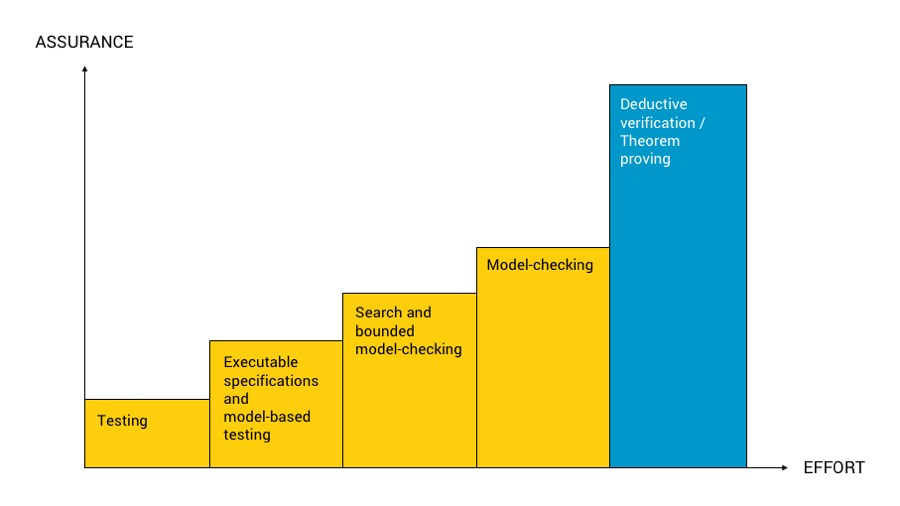
\includegraphics[width=\linewidth]{assets/verification.png}
  \caption{Different verification methods and how they generally compare with respect to the confidence-effort trade off.}
  \label{fig:verification}
\end{figure}

As the diagram indicates, the strongest guarantees, and thus the highest degree of trustworthiness, are obtained through deductive verification and theorem proving. In deductive verification, systems are modeled and specified inside expressive formal logical systems, and verified in a similar way to how mathematicians prove theorems - in principle by elaborating proofs of statements step-by-step. Among tools for deductive verification, \emph{proof assistants} offer the smallest trusted computing base necessary to trust verified statements, realized in modestly-sized trusted checkers that only assume a small set of axioms accepted by most mathematicians. Although they provide such strong guarantees, proof assistants can offer extensive automation and user support. Nevertheless, the process of figuring out what properties are relevant, how these properties are specified and building up their proofs normally requires a great deal of human ingenuity and experience. However, once everything is specified, proofs developed in proof assistants can be machine-checked, and persisted to serve as independently verifiable evidence that the properties hold for the given system.

\subsection{Coq and the Mathematical Components Library}

Coq is a proof assistant based on type theory, developed for more than 30 years. Coq can be viewed as consisting of, on the one hand, a small and powerful purely functional programming language, and on the other hand, a system for specifying and proving properties. A Coq user writes functions and data and then interactively constructs the proof of a theorem by trying different proof tactics that transform the state of the in-progress proof. Coq only accepts the theorem after its checker has been run on the purported proof. Coq has previously been used to develop a verified C compiler, formally prove mathematical results such as the four-color theorem, and verify distributed protocols (see, for example, our previous Casper formal verification effort for the Ethereum Foundation).

[Mathematical Components]

%We employ several existing Coq libraries which already formalized
%the majority of the mathematics we need to define and reason about Casper.
%Mathematical Components~\cite{MathComp} is a Coq library based on packaging
%mathematical structures and results in the form of Coq \emph{canonical
%  structures}, which can be reused and specialized when
%required~\cite{Garillot2009}.
%The library was used by Gonthier~et~al.\ to capture finite group theory and
%prove fundamental results in abstract algebra~\cite{Gonthier2013}.
%In addition to structures from abstract algebra, the library also contains
%encodings of and results about many standard data structures, such as numbers,
%lists, and finite sets.


\section{Modeling and Verification Approach}
\label{sec:approach}

[TODO: Karl]
We developed a model of the Algorand consensus protocol in Coq, and proved a slew of its properties that we then used to ultimately show the asynchronous safety property. In total, our Coq development contains around 2000 lines of Gallina code for the specification of the model and its properties, and around 4000 lines of proof scripts that build the formal proofs. The source files also contain almost 1000 lines of comments that motivate and explain the specifications and lemmas.

The modeling effort involved primarily:
\begin{itemize}
\item Defining all the needed data types and structures, such as message types and records, using the inductive constructions facilitated by the logic underlying Coq. Definitions were designed to utilize various existing infrastructure components, provided as Coq libraries, including most prominently the Mathematical Components (MathComp) library. These definitions specify the structure of the protocol’s state.
\item Defining both: (1) utility functions, such as computing the number of soft-votes seen by a user so far or identifying the proposal with the least credential, and (2) logical propositions asserting, for example, the preconditions for a cert-voting action or whether some event (like cert-voting) had taken place along an execution path. Functions and propositions constitute the basic building blocks using which other more complex (inductive) definitions and statements are formed.
\item Stating and proving basic structural properties about these definitions to ensure their correctness with respect to their intended behavior, for example, showing that a defined relation is a complete order or that a function that updates user timers preserves the set of users in the system. These properties are crucial for building up other proofs of more elaborate statements. We note that definitions imported from external libraries, such as MathComp, come equipped with many useful properties already proved, which are also heavily used in our model.
\item Formalizing the argument for safety and proving the safety theorem, which in turn required designing a proof plan and identifying the intermediate results that will need to be shown as proof obligations. This process is iterative, since many intermediate results were deep enough that they required breaking them down into smaller, more manageable pieces. The whole process was guided by the informal proof arguments documented in the protocol description by Algorand[add pointers]. We highlight some of the details of this proof later in the report.
\end{itemize}

\subsection{The State Transition Relation}
At the heart of the model is the global state transition relation (GTransition defined here[add link] and denoted \lstinline{g ~~> g'}, where $g$ and $g'$ are global states of the protocol). This relation defines inductively how the protocol's global state transitions into another state in one step. For example, the global state may transition into another by advancing time, having one of its users make an internal transition or by having the adversary partition the network, and so on. Each transition is guarded by certain preconditions that need to be satisfied for the transition to be enabled. Therefore, the statement that \lstinline{g ~~> g'} tells us that the preconditions for one of these global transition cases were enabled and that transition was taken to transform $g$ into $g'$.

Most statements asserting that some kind of event has taken place are specified as propositions on traces, possibly satisfying certain conditions. A trace is a non-empty sequence of global states that is built up using the global transition relation, i.e. if state $g_i$ is the $i$th state in the sequence and $g_{i+1}$ is the $(i+1)$th state, then the ordered pair $g_i$ and $g_{i+1}$ belongs to the global transition relation. 

[add diagram]

By specifying path properties as propositions on traces, we are able to define generically what the property is without having to assume a concrete initial state (or a set of initial states). Any conditions required for the property to hold can be specified as constraints on the states of the trace being considered.

For example, the property that a block was certified in a period is captured by the proposition:

\begin{lstlisting}[language=Coq]
Definition certified_in_period trace r p v :=
  exists (certvote_quorum:{fset UserId}),
     certvote_quorum `<=` committee r p 3
  /\ #|` certvote_quorum | >= tau_c
  /\ forall (voter:UserId), voter \in certvote_quorum ->
       certvoted_in_path trace voter r p v.
\end{lstlisting}

It states that the proposition holds for a trace if there exists a large-enough quorum of users selected for cert-voting who actually published cert-votes along that trace for the given period (the proposition \lstinline{certvoted_in_path}).

\subsection{Assumptions}

Most formalizations of programs and protocols are parameterized in specific ways, to be valid across a wide range of configuration choices and scenarios that may occur in practice. Our Algorand model is parameterized on a finite set of users (e.g., network nodes), and on a finite set of values used in message payloads (representing blocks and block hashes). 

\begin{lstlisting}[language=Coq]
Parameter UserId : finType.
Parameter Value : finType.
\end{lstlisting}

Values are assumed to be checkable for validity. We also consider an arbitrary, but totally ordered, datatype of credentials owned by users, and assume there is some way, given a credential, to say whether its owner is a committee member. Finally, we parameterize on delays and Algorand-specific configuration parameters such as number of votes required to move between periods. For example, this parameter represents the message delivery delay:

\begin{lstlisting}[language=Coq]
Parameter lambda : R.
\end{lstlisting}

Besides these and other parameters (16 in total), we also express assumptions, most related to our parameters, in the form of axioms. We use four kinds of axioms: 
\begin{enumerate}
\item Standard axioms from classical logic. We use these axioms (three in total) to facilitate simpler use of and reasoning about real numbers.

\item Axioms about credentials (two in total), such as about their uniqueness across different users (the symbol <> means “not equal”, and the arrow “->” denotes logical implication): 

\begin{lstlisting}[language=Coq]
Axiom credentials_different :
  forall (u u' : UserId) (r r' : nat) (p p' : nat) (s s' : nat),
  u <> u' -> credential u r p s <> credential u' r' p' s'.
\end{lstlisting}

This axiom states that any two distinct user identifiers u and u’ will have distinct credentials no matter what the round, period and step values are.

\item Axioms on limits of message delays (two in total), such as the axiom specifying how the small message delivery delay lambda, block message delivery delay \lstinline{big_lambda} and the recovery time period L are all related:

\begin{lstlisting}[language=Coq]
Axiom delays_order : (3 * lambda <= big_lambda < L)%R.
Axiom delays_positive : (lambda > 0)%R.
\end{lstlisting}

\item Axioms on the composition of groups (quorums) of users satisfying certain conditions. For example, the assumption that “any two large-enough cert-voting committees for a given round-period-step triple must share at least one honest user“, which captures the honest supermajority assumption in Algorand for the cert-voting case, is specified as:

\begin{lstlisting}[language=Coq]
Axiom quorums_c_honest_overlap : quorum_honest_overlap_statement tau_c.
\end{lstlisting}

where \lstinline{quorum_honest_overlap_statement} is a definition parameterized by the committee size threshold value tau:

\begin{lstlisting}[language=Coq]
Definition quorum_honest_overlap_statement (tau : nat) : Prop :=
  forall (trace : seq GState) (r p s : nat) (quorum1 quorum2 : {fset UserId}),
    quorum1 `<=` committee r p s ->		
    // quorum1 is a subset of the committee of r-p-s
    #|` quorum1 | >= tau ->					
    // quorum1 is at least as large as the threshold tau
    quorum2 `<=` committee r p s ->		
    // quorum2 is a subset of the same committee 
    #|` quorum2 | >= tau ->					
    // quorum2 is at least as large as the threshold tau
    exists honest_voter,
      honest_voter \in quorum1
      /\ honest_voter \in quorum2
      /\ honest_during_step (r,p,s) honest_voter trace.
\end{lstlisting}

\lstinline{quorum_honest_overlap_statement} defines a proposition that holds if for any two quorums of users, each of size at least tau, and who are all committee members for the given r-p-s triple, there is an honest user for the step r-p-s who belongs to both quorums. In total, there are six axioms of this kind.
\end{enumerate}

Our axioms either capture statements accepted by most mathematicians (1 above) or assumptions made by Algorand designers on the runtime environment (2-4 above).

%This section outlines our approach to modeling and verifying Casper in Coq.
%
%We decided to translate Hirai's Casper definitions and theorems~\cite{pos} from
%Isabelle/HOL to Coq, and connect the resulting Casper definitions with key
%definitions from Toychain.
%At the same time, we leveraged the Toychain definitions and results to capture
%the behavior of nodes as found in the Casper-based beacon chain for
%Ethereum~\cite{Beacon}.
%For tractability, we focused on translating and adapting Hirai's formal models
%with a \emph{static} validator set, which are simpler (but less realistic) than
%the corresponding models with churn among validators.
%
%We used concepts from the Mathematical Components library as far as possible.
%In particular, validators are identified by fixed-size keys so
%we represent validators as members of a \emph{finite type}
%(having a finite number of members that can be enumerated), written
%\lstinline{Validator : finType}.
%Using the library's \lstinline{finType} simplifies forming and reasoning about sets of
%validators.
%
%%\subsection{From Isabelle/HOL to Coq}
%Since the formal model for establishing safety by Hirai mostly uses first-order
%reasoning, we were able to successfully leverage the CoqHammer
%extension~\cite{Czajka2018,CoqHammer} to perform proofs in Coq that closely
%followed Isabelle/HOL proofs.
%At the same time, we reformulated Isabelle locale variables to Coq section variables.
%
%In particular, the assumption on abstract set membership becomes:
%\begin{lstlisting}[language=Coq]
%Variables quorum_1 quorum_2 : {set {set Validator}}.
%Hypothesis qs : forall q1 q2, q1 \in quorum_1 -> q2 \in quorum_1 ->
% exists q3, q3 \in quorum_2 /\ q3 \subset q1 /\ q3 \subset q2.
%\end{lstlisting}
%\lstinline{quorum_1} abstracts the collection of sets of validators with
%combined deposits (``weight'') of at least $\frac{2}{3}$ of the total.
%A link will be justified if every validator in some set in \lstinline{quorum_1}
%has voted for the link.
%\lstinline{quorum_2} abstracts the collection of sets of validators with
%combined deposits of at least $\frac{1}{3}$ of the total.
%Casper safety proofs generally show that an attack cannot succeed without
%a set of attacking validators of at least this size being slashed for it.
%
%To abstract a block forest, we assume a parent relationship on a type
%\lstinline{Hash} (with member \lstinline{genesis}).
%\begin{lstlisting}[language=Coq]
%Variable hash_parent : rel Hash.
%Hypothesis hash_at_most_one_parent : forall h1 h2 h3,
% hash_parent h2 h1 -> hash_parent h3 h1 -> h2 = h3.
%\end{lstlisting}
%Given the block forest we define the global state as a function which represents
%votes cast by validators:
%\begin{lstlisting}[language=Coq]
%Record State :=
% mkSt { vote_msg : Validator -> Hash -> nat -> nat -> bool }.
%\end{lstlisting}
%The arguments are the validator making the vote, the hash and height of the
%target block, and the height of the source block.
%Blocks have at most one parent so the source hash of any valid vote can be
%computed.
%
%With votes defined we can then define the slashing conditions of Casper (shown
%in Figure~\ref{fig:slashing-conditions}) in terms of conflicting votes, and define
%a predicate saying a validator is slashed in a given global state.
%\begin{figure}
%\textsc{An individual validator $v$ must not publish two distinct votes},
%\[\langle v,s_1,t_1,h(s_1),h(t_1)\rangle \qquad \textsc{and} \qquad \langle v,s_2,t_2,h(s_2),h(t_2) \rangle,\]
%\textsc{such that either}:
%\begin{description}
%\item[\phantom{I}I.] $h(t_1) = h(t_2).\quad$
%  Equivalently, a validator must not publish two distinct votes for the same
%  target height.
%\item[II.] $h(s_1)<h(s_2)<h(t_2)<h(t_1).$
%  Equivalently, a validator must not vote within the span of its other votes
%\end{description}
%\caption{Slashing Conditions of Casper}\label{fig:slashing-conditions}
%\end{figure}
%\begin{lstlisting}
%Definition slashed_dbl_vote s n :=
% exists h1 h2, h1 <> h2 /\ exists v s1 s2,
%   vote_msg s n h1 v s1 /\ vote_msg s n h2 v s2.
%\end{lstlisting}
%Condition I is violated if validator \lstinline{n} has voted for two edges
%targeting different blocks \lstinline{h1} and \lstinline{h2} at height \lstinline{v}.
%\begin{lstlisting}
%Definition slashed_surround s n :=
%  exists h1 h2 v1 v2 s1 s2, v1 > v2 /\ s2 > s1
%    vote_msg s n h1 v1 s1 /\ vote_msg s n h2 v2 s2.
%\end{lstlisting}
%Condition 2 is violated if validator \lstinline{n} has made two votes so the
%source height \lstinline{s1} and target height \lstinline{v1} of one strictly
%surround the source height \lstinline{s2} to target height \lstinline{v2}
%range of the other vote.
%\begin{lstlisting}
%Definition slashed s n : Prop :=
% slashed_dbl_vote s n \/ slashed_surround s n.
%\end{lstlisting}
%A validator is slashed if it has violated either slashing condition.
%
%We can also define justified links between blocks based on the votes in a state:
%\begin{lstlisting}[language=Coq]
%Definition justified_link s q parent pre new now :=
%  q \in quorum_1 /\ (forall n, n \in q -> vote_msg s n new now pre) /\
%  now > pre /\ nth_ancestor (now - pre) parent new.
%\end{lstlisting}
%The conjuncts respectively require that set \lstinline{q} is large enough to
%justify a link, that every validator in \lstinline{q} has voted for this link,
%that the claimed height \lstinline{now} of the target is greater than the
%claimed height \lstinline{pre} of the source, and that \lstinline{parent} is
%actually the ancestor the appropriate number of levels above \lstinline{new}.
%
%This allows us to define justified blocks, starting from the genesis block, and
%furthermore finalized blocks, as in the Casper paper.
%\begin{lstlisting}
%Inductive justified : State -> Hash -> nat -> Prop :=
%| orig : forall s, justified s genesis 0
%| follow : forall s parent pre q new now,
%    justified s parent pre ->
%    justified_link s q parent pre new now ->
%    justified s new now.
%\end{lstlisting}
%\begin{lstlisting}
%Definition finalized s q h v child := justified s h v
%  /\ h <~ child /\ justified_link s q h v child v.+1.
%\end{lstlisting}

\section{The Safety Theorem}
\label{sec:safety}

[TODO: Brandon] 
The safety theorem says that only one block may be certified in a round, which means the blockchain will not fork. The key assumptions of the proof are some properties of cryptographic self-selection. We have not formalized the cryptographic reasoning, or the notion of negligible probability, and instead simply assume that it's impossible to have a quorum of committee members without enough honest members.

The statement of the theorem says that any two certificates from the same round must be for the same block:

\begin{lstlisting}[language=Coq]
Theorem safety : forall (g0:GState) (trace:seq GState) (r:nat),
  state_before_round r g0 ->
  is_trace g0 trace ->
  forall (p1:nat) (v1:Value), certified_in_period trace r p1 v1 ->
  forall (p2:nat) (v2:Value), certified_in_period trace r p2 v2 ->
  v1 = v2.
\end{lstlisting}


Note the preconditions \lstinline{state_before_round r g0}, which states that the trace goes back long enough in history when no user has yet entered round r, and \lstinline{is_trace g0 trace}, which states that the trace is a valid trace beginning at g0, obtained by the transitive closure of the global transition relation.

When there is a "network partition" allowing the adversary to delay messages, it's possible to end up with certificates from multiple periods if cert-vote messages are delayed enough for some nodes to advance to the next period, but these certificates will still all be for the same block.

The proof of the main safety theorem above[LINK safety] first considers two cases, for whether the two certificates are from the same period or different periods.

The case when the certificates are in the same period is handled in the lemma \lstinline{one_certificate_per_period}. This proof uses the quorum hypothesis to conclude that there is an honest node that contributed a cert-vote to both quorums, and the lemma \lstinline{no_two_certvotes_in_p} shows that an honest node cert-votes at most once in a period, by analyzing all the steps of the protocol.

The case of different periods is proved using an invariant, which holds for the period that produces the first certificate and for all later periods in the same round. The invariant is defined in \lstinline{period_nextvoted_exclusively_for}, and says that no step of these periods produce a quorum of open next-votes, and any quorum of next-votes is for the same value that the first
certificate was for.

Lemma \lstinline{certificate_is_start_of_next_period} shows that this is true of next votes from the period that produced the first certificate,
Lemma \lstinline{excl_enter_excl_next} shows that if this is true for one period, it is true for the next.
Lemma \lstinline{prev_period_nextvotes_limits_cert_vote} shows that if the invariant holds for one period then any certificate produced in the next period can only be for the same value.

The lemma \lstinline{certificate_is_start_of_next_period} is the only place we need to use a more complicated quorum hypothesis. Intuitively, if committee members are selected approximately randomly from the full population of users, so if some property (unrelated to committee
membership) is true for all honest members of one quorum, then it's almost
certainly true of most honest users overall, and even for a later step there
cannot be another quorum where none of the honest members have that property.

The specific property we consider is that the user had seen a quorum of soft-votes
for value v by the end of the cert-voting step of the period where the first
certificate was produced.
This is a precondition for making an honest cert-vote, so this property is
true for all honest users whose vote is part of the certificate.
Then by the interquorum assumption we have that most honest users will have
seen a quorum of soft-votes for v, and any quorum of next-voters from this period
has at least one honest user that saw a quorum of soft-votes for v.
By the preconditions for next-voting this honest user could only have next-voted for v,
so the invariant is established.

To prove the latter two lemmas \lstinline{excl_enter_excl_next} and
\lstinline{prev_period_nextvotes_limits_cert_vote}
we consider that any quorum of next-votes or cert-votes contains an honest voter, and looking at the preconditions for an honest node to make a cert-vote or next-vote.
In both cases the vote can only be for v because we know from
the invariant that any quorum of soft-votes in the new period are votes for v by \lstinline{prev_period_nextvotes_limits_honest_soft_vote},
and that our honest node hasn't received a quorum of open next-votes from
the previous period by lemma
\lstinline{no_bottom_quorums_during_from_nextvoted_excl}.
\lstinline{prev_period_nextvotes_limits_honest_soft_vote} is proven in turn by
looking at the rules for an honest node to advance to a new period to establish than the node got "starting value" v, and with that starting value it cannot soft-vote anything but v unless it has also seen a quorum of open next-votes.

%This section describes the Coq formalization and verification of
%Casper's \emph{accountable safety} property.
%A major part of the Casper design is ensuring that an attack cannot
%finalize blocks on both sides of a fork in the chain without the
%attacker losing a significant amount of money by having their validator deposits slashed.
%This is formalized as the accountable safety theorem, which says that if two
%blocks are finalized and neither is an ancestor of the other, then validators
%having at least $\frac{1}{3}$ of the deposits must have violated the slashing
%conditions.
%The difference between slashing violations and actually losing funds is
%addressed and handled with other countermeasures in the Casper
%paper~\cite{Buterin2017}.
%
%Let \lstinline{hash_ancestor} be the reflexive-transitive closure of the
%\lstinline{hash_parent} relation.
%Building on the definitions of validator quorums and justification described above,
%we define a fork in a state as two conflicting finalized blocks (hashes):
%\begin{lstlisting}[language=Coq]
%Definition fork s := exists h1 h2 q1 q2 v1 v2 c1 c2,
% finalized s q1 h1 v1 c1 /\ finalized s q2 h2 v2 c2 /\
% ~ hash_ancestor h2 h1 /\ ~ hash_ancestor h1 h2 /\ h1 <> h2.
%\end{lstlisting}
%With \lstinline{slashed s v} capturing that the slashing conditions
%in Figure~\ref{fig:slashing-conditions} are true in state \lstinline{s} for
%validator \lstinline{v}, we define the condition of $\frac{1}{3}$ of validators
%by weight being slashed:
%\begin{lstlisting}[language=Coq]
%Definition quorum_slashed s :=
% exists q, q \in quorum_2 /\ forall v, v \in q -> slashed s v.
%\end{lstlisting}
%This allows us to define and prove accountable safety:
%\begin{lstlisting}[language=Coq]
%Theorem accountable_safety : forall s, fork s -> quorum_slashed s.
%\end{lstlisting}
%The proof roughly follows the informal argument~\cite{Buterin2017}.
%If the two finalized blocks were at the same height then
%at least $\frac{1}{3}$ weight (or a \lstinline{quorum_2} set)
%of validators violated slashing condition I.
%Otherwise, consider the path of justified links which justifies
%the higher finalized block.
%If any justified block along this path has the same height
%as the other justified block or its justified immediate child
%then we again have a sufficiently large set of
%validators violating slashing condition I.
%Otherwise find the justified link along that path with
%a source lower than the other justified block and a target
%higher than its child.
%Taking this link along with the justified link between the lower
%finalized its child we have a set of validators violating
%slashing condition II.
%
%% The final step is analysis of two cases. In the first case, the validators
%% of the two finalized blocks are distinct:
%% \begin{lstlisting}[language=Coq]
%% Lemma case_1 : forall s q1 q2 h1 v1 x h2 v2 xa,
%%  finalized s q1 h1 v1 x -> finalized s q2 h2 v2 xa ->
%%   ~ hash_ancestor h2 h1 -> h1 <> h2 -> v1 > v2 ->
%%   quorum_slashed s.
%% \end{lstlisting}
%% In the second case, they are one and the same:
%% \begin{lstlisting}[language=Coq]
%% Lemma case_2 : forall s q1 h1 v1 x q2 h2 xa,
%%  finalized s q1 h1 v1 x -> finalized s q2 h2 v1 xa ->
%%  h1 <> h2 -> quorum_slashed s.
%% \end{lstlisting}
%
%%The key lemma
%%  finalized s q1 h1 v1 c1 ->
%%  finalized s q2 h2 v2 c2 ->
%%  h2 </~* h1 ->
%%  h1 </~* h2 ->
%%  h1 <> h2 ->
%%  quorum_slashed s.
%
%%Then the safety property is stated as saying that a
%%fork can only exist in a state if some \lstinline{quorum_2}
%%set of validators has been slashed:
%
%%A block defined by the hash \lstinline{h} is justified
%%at a distance \lstinline{d} from the genesis block if
%%there is
%%
%%%justified s parent pre ->
%%%justified_link s q parent pre h now ->
%%
%%\begin{lstlisting}[language=Coq]
%%Definition finalized s q h v c := hash_parent h c /\
%% justified s h v /\ justified_link s q h v c v.+1.
%%\end{lstlisting}
%
%%\begin{lstlisting}[language=Coq]
%%fork s ->
%%\end{lstlisting}
%%Intuitively, this property states that a fork cannot arise unless
%%at least $\frac{1}{3}$ weight of validators misbehaved, and
%%that if a fork does happen then at least $\frac{1}{3}$ of the
%%malicious validators had their deposits slashed.
%%The proof follows the informal argument~\cite{Buterin2017}.
%
%\section{Plausible Liveness}
%\label{sec:liveness}
%The liveness goal for Casper is that as long as at least $\frac{2}{3}$ of validators
%are following the protocol and block proposals continue, then further checkpoints
%can continue to be finalized regardless of the behavior of the less the $\frac{1}{3}$
%of misbehaving validators, without needing any of the honest validators to violate a
%slashing condition and sacrifice their deposit to allow the chain to live.
%
%Our Coq proof is based on the argument given in~\cite{Buterin2017}, and also
%Yoichi Hirai's Isabelle/HOL proof of plausible liveness for an older variant
%of the Casper protocol~\cite{pos}.
%
%\subsection{Context}
%The proof works with the same model of checkpoint blocks as the accountable
%safety proof.
%We are given a set of checkpoint block hashes, a parent relationship giving each
%hash at most one parent, and a hash of the genesis block.
%The changing part of the system states is only the set of votes,
%because we do not model the block proposal process or dynamic validator sets.
%
%
%Finalization is an essential part of the Casper design for dynamic validator sets,
%which uses finalized blocks as the boundary of the ``epochs'' where the validator
%set can change.
%Because of this essential role we state and prove liveness in terms of
%a hash and height of the most recent previously-finalized block, even though
%we are not yet proving liveness in the presence of dynamic validator sets.
%\begin{lstlisting}
%Variable epoch_start : Hash.
%Variable epoch_height : nat.
%Hypothesis epoch_ancestry :
%  nth_ancestor epoch_height genesis epoch_start.
%\end{lstlisting}
%Here \lstinline{epoch_start} is the hash of that block, \lstinline{epoch_height}
%is its height, and \lstinline{epoch_ancestry} is a proof that the epoch start block
%is actually at the claimed height over the genesis block.
%
%To demonstrate a further block can be finalized we only need to consider justification
%of blocks descending from the start of this epoch.
%We define justification within the epoch as having a path of super-majority links
%from the epoch start up to a block.
%\begin{lstlisting}
%Inductive justified_this_epoch (st:State)
%  : Hash -> nat -> Prop :=
%| epoch_justified :
%    justified_this_epoch st epoch_start epoch_height
%| justfied_link : forall s s_h t t_h,
%    justified_this_epoch st s s_h ->
%    hash_ancestor s t ->
%    supermajority_link st s t s_h t_h ->
%    justified_this_epoch st t t_h.
%\end{lstlisting}
%This definition defines justification inductively, from two cases.
%A block is justified if it is the epoch start block,
%or if it has a justified ancestor and a supermajority of validators
%have voted for a link to this block from that ancestor.
%
%Besides the parameterization over the epoch start block,
%we do not actually consider the history of any past epochs.
%In particular, we assume that the well-behaved nodes have not made any
%votes with sources outside the current epoch.
%We could work without that assumption, but we would need to repeat
%part of the accountable safety proof to argue that an unslashed
%validator's votes from past epochs cannot prevent them from
%safely making the votes chosen in out proof.
%
%\subsection{Theorem}
%To formalize a statement of plausible liveness, we follow our examples and
%abstract away from any implementation details of ``following the protocol'',
%and simply require that our $\frac{2}{3}$ good validators have not made certain
%sorts of bad votes.
%For the conclusion we also ignore the details of how validators decide to make
%votes, and simply show that there is some set of votes which the good validators
%could make that would finalize a further block and not violate slashing conditions.
%
%In Hirai's proof for the previous Casper design it was sufficient to simply require
%that the good validators were unslashed.
%The current Casper design intentionally removed any slashing conditions that required
%knowing the state of the chain when the votes were made.
%We found that \emph{one of these conditions was essential to the proof}, so our definition
%of good behavior for the current Casper protocol requires that a validator has not
%made votes with an unjustified source in addition to requiring that a good validator
%had not been slashed.
%
%We define the condition that a super-majority of validators is good given a set of votes:
%\begin{lstlisting}
%Definition two_thirds_good (st : state) :=
%  exists good_validators, good_validators \in quorum_1
%  /\ forall v, v \in good_validators
%     -> (~ slashed st v /\ sources_justified st v).
%\end{lstlisting}
%The property \lstinline{sources_justified st v} says the source block of any
%vote that validator \lstinline{v} has made in state \lstinline{st} is justified
%within the current epoch\footnote{This enforces the assumption above that
%good nodes only have votes with sources within the current epoch}
%\begin{lstlisting}
%Definition sources_justified st v :=
%  forall s t s_h t_h,
%    vote_msg st v s t s_h t_h ->
%    hash_ancestor epoch_start s /\ justified_this_epoch st s s_h.
%\end{lstlisting}
%
%The other explicit hypothesis of our plausible liveness theorem
%captures the assumption that block proposals continue.
%We only need to assume that blocks can be found above the
%highest justified block, but we may need to find a block at arbitrary
%height.
%These definitions capture the properties of being the highest
%justified block (which will be unique by accountable safety),
%and having descendants at arbitrary heights.
%\begin{lstlisting}
%Definition blocks_exist_high_over (base : Hash) : Prop :=
%  forall n, exists block, nth_ancestor n base block.
%Definition highest_justified st b b_h : Prop :=
%  forall b' b_h', b_h' >= b_h
%  -> justified_this_epoch st b' b_h'
%  -> b' = b /\ b_h' = b_h.
%\end{lstlisting}
%
%With these ingredients, this is the statement of plausible liveness
%that we prove:
%\begin{lstlisting}
%Lemma plausible_liveness :
%  forall st, two_thirds_good st ->
%  (forall b b_h, highest_justified st b b_h
%     -> blocks_exist_high_over b) ->
%  exists st', unslashed_can_extend st st'
%   /\ no_new_slashed st st'
%   /\ exists (new_finalized new_final_child:Hash) new_height,
%        justified_this_epoch st' new_finalized new_height
%         /\ epoch_height < new_height
%         /\ new_finalized <~ new_final_child
%         /\ supermajority_link st' new_finalized new_final_child
%                                   new_height new_height.+1.
%\end{lstlisting}
%
%The desired conclusion of the theorem is expressed by stating that
%there exists a set of votes \lstinline{st'},
%such that any votes which were not already in \lstinline{st} were
%made by unslashed validators,
%that no validators that were unslashed in \lstinline{st}
%are slashed in \lstinline{st'},
%and that there is a block \lstinline{new_finalized} which is
%finalized under votes \lstinline{st'} and is higher than
%the previous finalized block.
%
%The proof proceeds as outlined in~\cite{Buterin2017}:
%We take the highest justified checkpoint J which is a descendant of the most
%recently finalized block, consider the maximum height of the target of any
%existing vote, and use the assumption that block proposals continue to
%find a descendant A of J at a greater height than that, and an immediate child B of A.
%Then all good validators will vote for the links J$\rightarrow$A and A$\rightarrow$B.
%This is easily shown to finalize A and require votes only from good validators.
%It remains only to prove that this does not violate any slashing condition.
%Recall the definitions of the slashing conditions from Figure~\ref{fig:slashing-conditions}.
%\begin{itemize}
%\item
%Condition I is not violated because a good validator's two new votes have
%targets at different heights, and any previous votes have a target at a lower height
%than A, by choice of A.
%\item
%Condition II is not violated because the two new votes of good validators do not nest,
%a previous vote cannot have a range surrounding a new vote because all previous votes
%have targets below A by choice of A,
%and a previous vote cannot nest within the vote for J$\rightarrow$A because it would
%have a source above J, we assume existing votes from good validators have justified
%sources, and J is the highest justified block.
%\end{itemize}
%
%\subsection{Unslashed is not enough}
%One might wonder if a different voting strategy could prove plausible
%liveness while only needing to require that the good validators be unslashed.
%To show that there cannot be such a proof, we give an example where all
%validators are unslashed but it is impossible to justify any further blocks
%(let alone finalize a further block).
%Every validator in this example has made one vote with an unjustified source.
%
%\begin{figure}[h]
%\begin{tikzpicture}[node distance=5mm,
%      terminal/.style={rectangle,draw=black,rounded corners=1mm}]
%\node (F) [terminal] {$F$};
%\node (A1) [terminal,above left=of F] {$A_1$};
%\node (A2) [terminal,above=of A1] {$A_2$};
%\node (B1) [terminal,above right=of F] {$B_1$};
%\node (B2) [terminal,above=of B1] {$B_2$};
%\graph {
%  (F) ->[dotted] (A1) ->[dotted] (A2);
%  (F) ->[dashed] (B1) ->[dashed] (B2);
%};
%\end{tikzpicture}
%\caption{Unslashed Progress Counterexample}\label{fig:unslashed-counterexample}
%\end{figure}
%The example is shown in Figure~\ref{fig:unslashed-counterexample}.
%$F$ is the most recent finalized block, $A_1$ and $B_1$ immediate children of $F$,
%and $A_2$ and $B_2$ immediate children (respectively) of $A_1$ and $A_2$.
%Half of the validators have voted for the edges $F\!\!\rightarrow\!\! A_1$
%and $A_1\!\! \rightarrow\!\! A_2$ (dotted arrows) and the other half of
%the validators have voted for $F\!\! \rightarrow\!\! B_1$
%and $B_1\!\! \rightarrow\!\! B_2$ (dashed arrows).
%It is impossible to make a super-majority link from $F$ to any other block
%without some validators being slashed.
%A new edge from $F$ to a block one or two levels above $F$ would violate slashing
%Condition I, because every validator already has votes with a target at that level.
%An edge from $F$ to a block at any higher level would violate Condition II,
%with the inner vote being that validator's vote for $A_1\!\! \rightarrow\!\! A_2$
%or $B_1\!\! \rightarrow\!\! B_2$.
%
%\section{Instantiating Hypotheses and Parameters}
%
%The definitions and proven properties in the abstract
%models of Casper are quite far from those in the Casper paper~\cite{Buterin2017},
%partly due to proof engineering concerns described above.
%To bring our results closer to the paper, and thus to actual implementations,
%we instantiate the key abstractions.
%In particular, we assume an arbitrary function which maps validators to their deposits:
%\begin{lstlisting}[language=Coq]
%Variable deposit : Validator -> nat.
%\end{lstlisting}
%Using the support for big operators in Mathematical Components~\cite{Bertot2008}, we
%then define the total deposits of all validators:
%\begin{lstlisting}[language=Coq]
%Definition deposits := \sum_(v : Validator) (deposit v).
%\end{lstlisting}
%We also define a function from a natural number \lstinline{n} to the set of sets of
%validators which have total deposit at least \lstinline{n}:
%\begin{lstlisting}[language=Coq]
%Definition gdset n := [set x in powerset [set: Validator] |
% \sum_(v in x) (deposit v) >= n].
%\end{lstlisting}
%Writing \lstinline{m %/ d} for the quotient of the Euclidean division of
%\lstinline{m} by \lstinline{d}, we define two sets:
%\begin{lstlisting}[language=Coq]
%Definition deposit_bot := gdset (deposits %/ 3).+1.
%Definition deposit_top := gdset ((2 * deposits) %/ 3).+1.
%\end{lstlisting}
%which allows us to prove:
%\begin{lstlisting}[language=Coq]
%Lemma deposit_validator_intersection : forall q1 q2,
% q1 \in deposit_top -> q2 \in deposit_top ->
% exists q3, q3 \in deposit_bot /\ q3 \subset q1 /\ q3 \subset q2.
%\end{lstlisting}
%using the arithmetical lemma
%\begin{lstlisting}[language=Coq]
%Lemma thirds : forall n, (n %/ 3).+1 + n <= 2 * (2 * n %/ 3).+1.
%\end{lstlisting}
%This intersection lemma shows that we can instantiate the
%abstract \lstinline{quorum_1} and \lstinline{quorum_2}
%used in our proofs with specific sets \lstinline{deposit_top}
%and \lstinline{deposit_bot}.
%
%\subsection{Block Trees and Transition System}
%
%Working from the other end of the abstraction spectrum, we define
%functions and datatypes in Coq resembling those in the beacon chain
%implementation~\cite{Beacon}, to be used when defining global system
%state and node-local behavior.
%In particular, following Toychain, we abstracted a block to a Coq record
%type containing, most notably, a hash of the previous block and a collection of attestations
%by validators:
%\begin{lstlisting}[language=Coq]
%Record Attestation := mkAR { distance_src : nat;
% attester : Validator; }.
%
%Record Block := mkB { parent_hash : Hash;
%  attestations : seq Attestation;
%  distance : nat; }.
%\end{lstlisting}
%Using notions from the FCSL PCM library~\cite{fcslpcm}, we then define block forests as finite maps
%from hashes to blocks:
%\begin{lstlisting}[language=Coq]
%Definition Blockforest := union_map Hash Block.
%\end{lstlisting}
%This allows us to instantiate a suitably concrete parent relation over hashes:
%\begin{lstlisting}[language=Coq]
%Definition hash_parent_bf (bf : Blockforest) : rel Hash :=
%[rel x y | (x \in dom bf) && (y \in dom bf) &&
% if find y bf is Some b then parent_hash b == x else false].
%\end{lstlisting}
%for which we can instantiate the desired hypothesis:
%\begin{lstlisting}[language=Coq]
%Lemma hash_parent_bf_eq : forall f h1 h2 h3,
% hash_parent_bf f h2 h1 -> hash_parent_bf f h3 h1 -> h2 = h3.
%\end{lstlisting}
%
%We can now consider a block forest as a concrete global state, and define
%a mapping from from block forests to a \lstinline{vote_msg} function:
%\begin{lstlisting}[language=Coq]
%Definition vote_msg_bf bf v h distance distance_src : bool :=
% if find h bf is Some b then
%  (distance b == distance) &&
%  ((mkAR distance_src v) \in attestations b)
% else false.
%\end{lstlisting}
%The initial state of the system is simply the finite map taking the genesis
%block hash to the genesis block:
%\begin{lstlisting}[language=Coq]
%mkSt (vote_msg_bf (#GenesisBlock \\-> GenesisBlock))
%\end{lstlisting}
%Finally, we define a transition system that given a block \lstinline{b}, updates
%the global state \lstinline{bf} with \lstinline{b}:
%\begin{lstlisting}[language=Coq]
%mkSt (vote_msg_bf (#b \\-> b \+ bf))
%\end{lstlisting}
%Accountable safety holds for every state in this transition system, and we
%believe it can serve as a specification for the Casper beacon chain
%implementation~\cite{Beacon}, and is closer to the level of detail needed
%generate a correct-by-construction implementation from the specification.
%
%\subsection{Beacon Node}
%The state of the beacon chain~\cite{Beacon} is split into two main parts, an
%active state and a crystallized state. The active state is updated every block,
%while the crystallized state is only updated according to a cycle length
%parameter of the protocol, which is set to 64 slots in the beacon chain
%implementation~\cite{Beacon}.
%
%In our Coq formulation, we define the state of a node in the beacon chain as a
%record containing the blockforest and this beacon chain state.
%It also includes other parameters of the system, such as the cycle length
%mentioned above.
%\begin{lstlisting}[language=Coq]
%Record State {Hash : ordType} :=
%  Node {
%    id : NodeId;
%    peers : peers_t;
%    blocks : Blockforest;
%    cstate : @CrystallizedState Hash;
%    astate : @ActiveState Hash;
%    (* set to 1024 shards, see beacon chain implementation *)
%    shardCount : nat;
%    (* set to 64 slots, see beacon chain implementation *)
%    cycleLength : nat;
%  }.
%\end{lstlisting}
%When a block arrives on a node, the crystallized and active states are updated
%via the state transition function specified in~\cite{Beacon}. The update of the
%crystallized state is where most of the Casper functionality occurs. Should the
%slot number of the block be at least 64 past the last recalculation slot, the
%crystallized state is updated by applying the rewards and penalties for the
%validators, as well as managing the justification and finalization of blocks.
%For example, the Coq code for the state update has functions such as
%\lstinline{applyRewardsAndPenalties} below, which calculates and updates the
%balances for all active validators given the current state and block.
%
%\begin{lstlisting}[language=Coq]
%Definition applyRewardsAndPenalties
%           (crystallizedState :
%              @CrystallizedState [ordType of Hash])
%           (activeState : @ActiveState [ordType of Hash])
%           (blk : block)
%           (cycleLength : nat) :=
%  (* ... omitted ... *)
%\end{lstlisting}
%In addition to updating the crystallized and active states, the arrived block is
%also appended to the block forest, and the new state is returned, along with a
%message from the node that received the block to all of its peers.
%
%\begin{lstlisting}[language=Coq]
%Definition procInt (st : @State [ordType of Hash])
%           (tr : InternalTransition) (ts : Timestamp) :=
% let: Node n prs bf cst ast cl := st in
% match tr with
% | BlockT b =>
%   let: parentBlock := get_block bf (parent_hash b) in
%   let: (crystallizedState, activeState) :=
%      computeStateTransition cst ast parentBlock b cl in
%   let: newBf := bfExtend bf b in
%   pair (Node n prs newBf crystallizedState activeState cl)
%        (emitBroadcast n prs (BlockMsg b))
% end.
%\end{lstlisting}
%These definitions tighten the correspondence between our Coq code and the Beacon
%chain implementation in~\cite{Beacon}. Along with our abstract safety and
%liveness proofs, these definitions will allow us to perform verification at this
%low level, providing as much assurance as possible for the correctness of the
%Casper protocol.

\section{Conclusion}
\label{sec:conclusion}

The model we developed as part of this effort is generic, in that it captures the dynamics of the Algorand consensus protocol in a way that is orthogonal to the properties that we verify about it. This means that the model can be readily used to verify other properties of the system beyond asynchronous safety, including most importantly liveness. In fact, we anticipate that many of the smaller results shown about the protocol and used in the proof of safety will also constitute essential ingredients of the liveness proving effort. Nevertheless, proving liveness will probably require showing additional results, especially those related to timely message delivery and networking partitioning, which were not necessarily needed for the safety argument. But the model already has these components (time, message delays and network partitioning) and going into investigating liveness (and perhaps other properties) should be a seamless continuation of the effort involved in this project.


%Ongoing refinements include aligning the Toychain concept of a fork,
%which is in terms of block sequence prefixing, with the more abstract Casper
%notion of a fork in terms of finalized blocks over the closure of the parent
%hash relation.

%We presented a formalization of Casper in Coq, and proofs of accountable safety
%and plausible liveness.
%These proofs clarified the assumptions needed for the properties stated in
%the Casper paper~\cite{Buterin2017}, especially what assumptions on
%validator behavior are needed for plausible liveness.
%Our formalization work paves the way for transferring accountable safety and
%plausible liveness from Hirai's abstract models to hold for steps over the
%Toychain global state according to a step relation and node state definition
%matching those in the Ethereum reference beacon chain node
%implementation~\cite{Beacon}.

%Ultimately, we aim to transfer accountable safety and plausible liveness from
%Hirai's abstract models to hold for steps over the Toychain global state according to a step
%relation and node state definition matching those in the Ethereum reference beacon
%chain node implementation~\cite{Beacon}.
%
%That is, we will express and prove both properties
%along the lines of the \emph{clique consensus} property in Toychain~\cite{Pirlea2018}, i.e., similarly to
%\begin{lstlisting}[language=Coq]
%Theorem accountable_safety_inv : forall (w w' : World),
% accountable_safety w -> step w w' -> accountable_safety w'.
%\end{lstlisting}
%We then plan to use the step relation as a basis for a verified
%node implementation. We also want to capture \emph{sharded} systems,
%which consist of many separate blockchains for reasons of scalability~\cite{sharding}, and to keep up with the Casper protocol design, which is a moving target.

%\begin{lstlisting}[language=Coq]
%Theorem plausible_liveness : forall (w w' : World),
% accountable_safety w -> exists w', step w w' /\ new_justified w w'.
%\end{lstlisting}

%Our goal is to have our Coq implementation correspond as closely as
%possible with the implementation in~\cite{Beacon}. This gives us the greatest
%assurance that our proven properties hold in the most up-to-date Casper version.

%\begin{lstlisting}[language=Coq]
%Definition fork (bc1 bc2 : seq T) :=
% ~ (is_prefix bc1 bc2 \/ is_prefix bc2 bc1).
%\end{lstlisting}

%\section{Discussion}

%% Acknowledgments
\begin{acks}

We thank Jing Chen, Nickolai Zeldovich and Victor Luchango from Algorand for their help throughout the project. This work was funded by Algorand.

%                                        %% contents suppressed with 'anonymous'
%  %% Commands \grantsponsor{<sponsorID>}{<name>}{<url>} and
%  %% \grantnum[<url>]{<sponsorID>}{<number>} should be used to
%  %% acknowledge financial support and will be used by metadata
%  %% extraction tools.
%  This material is based upon work supported by the
%  \grantsponsor{GS100000001}{National Science
%    Foundation}{http://dx.doi.org/10.13039/100000001} under Grant
%  No.~\grantnum{GS100000001}{nnnnnnn} and Grant
%  No.~\grantnum{GS100000001}{mmmmmmm}.  Any opinions, findings, and
%  conclusions or recommendations expressed in this material are those
%  of the author and do not necessarily reflect the views of the
%  National Science Foundation.
\end{acks}


%% Bibliography
\bibliography{bib}


%% Appendix
%\appendix
%\section{Appendix}
%
%Text of appendix \ldots

\end{document}
